\documentclass[web]{uclthesis} % Options here are: final draft web
\RequirePackage{uclthesis}
% hepthesis documentation https://anorien.csc.warwick.ac.uk/mirrors/CTAN/macros/latex/contrib/hepthesis/hepthesis.pdf

% PDF metadata - not essential, but nice
\makeatletter
\@ifpackageloaded{hyperref}{%
  \hypersetup{%
    pdftitle = {SVS Thesis},
    pdfsubject = {SVS thesis},
    pdfkeywords = {
      Sam, Samuel, Van, Stroud, PhD, Thesis, ATLAS, Hbb, Higgs, GNN, Tracking, high, pT, transverse, momentum
    },
    pdfauthor = {\textcopyright\ Samuel Van Stroud}
  }
}{}
\makeatother

%% Define the thesis title and author
\title{Graph Neural Network Flavour Tagging and Boosted Higgs Measurements at the LHC}
\author{Samuel John Van Stroud\xspace}
\DeclareRobustCommand{\shortAuthor}{Samuel Van Stroud\xspace}
\date{\today}

%% Start the document
\begin{document}

%% Define the un-numbered front matter (cover pages, rubric and table of contents)
\begin{frontmatter}
  % Title
\titlepage[\UCL]%
{Submitted to \UCL in fulfilment\\
of the requirements for the award of the\\
degree of \PhD}

%% Declaration
\begin{declaration}
  I, \theauthor confirm that the work presented in this thesis is my own.
Where information has been derived from other sources, I confirm that
this has been indicated in the thesis.
\vspace*{3cm}
\begin{flushright}
\shortAuthor\hspace*{0.1\textwidth}\rule{0.5\textwidth}{0.25pt}
\end{flushright}

\end{declaration}

%% Abstract
\begin{abstract}
  no more than 300 words

This thesis presents work on improvement of the tracking and \btagging algorithms used by \ATLAS to perform \btagging at high transverse momenta.
Novel approaches, such as the classification of track origins and the application of graph neural networks have been successfully employed to markedly improve the \btagging performance at high \pt.
Work on analaysis of \Hbb decays was also performned using \SI{13}{\TeV} proton-proton collision data from the course of \runtwo.

\end{abstract}

%% Abstract
\begin{impactstatement}
  impact statement 500 words
\href{https://www.grad.ucl.ac.uk/essinfo/docs/Impact-Statement-Guidance-Notes-for-Research-Students-and-Supervisors.pdf}{link to ucl info}

\end{impactstatement}

%% Acknowledgements
\begin{acknowledgements}
  \DeclareRobustCommand{\personPH}{Peter Higgs\xspace}

Here is an example of how to declare commands for use in a single file that will not be needed elsewhere.
Additionally, it serves to illustrate the chapter referencing system.

Perhaps you might want to point out that \personPH provided helpful advice for \ChapterRef{chap:theory}.
\end{acknowledgements}

%% Preface
%\begin{preface}
%  You might want something generic about your experiment here and an overview of your work here.

The Large Hadron Collider (\LHC) is the largest and highest energy particle accelerator in the world, designed to collide protons with an unprecedented centre-of-mass energy of \unit{14}{\TeV} and instantaneous luminosity of \highL.
In addition, the \LHC has a heavy ion collision programme, aiming to collide lead nuclei with a centre-of-mass energy of \unit{5.5}{\TeV}.
In the early phase of operation, the proton-proton programme at the \LHC has been operating with reduced centre-of-mass energies of up to \unit{7}{\TeV}; these nevertheless represent the highest energy collisions that have yet been attained in a particle accelerator.

In this thesis, a number of separate analyses are presented, each aiming to probe our understanding of \QCD in this new energy regime, with $\rootS = \unit{7}{\TeV}$.
Differential \xs{s} of inclusive jets and \dijet{s} are performed across two orders of magnitude in jet transverse momentum and \dijet mass and are compared to next-to-leading order theoretical predictions.
Radiation between \dijet{s} is examined as a possible means of discriminating between DGLAP and \BFKL-like parton evolution schemes.

Finally, a more technical contribution to this thesis is a technique for ascertaining the uncertainty on the jet energy scale through intercalibration between jets in different regions of the detector.

%\end{preface}

%% ToC
\tableofcontents

%%% Technically UCL want these here - let's see if they care
%\listoffigures
%\listoftables

%% Strictly optional
%\frontquote%
%{God does not play dice with the universe; He plays an ineffable game of His own
%devising, which might be compared, from the perspective of any of the other
%players [i.e. everybody], to being involved in an obscure and complex variant of
%poker in a pitch-dark room, with blank cards, for infinite stakes, with a Dealer
%who won't tell you the rules, and who \emph{smiles all the time}.}
%{Terry Pratchett, \emph{Good Omens}}

\end{frontmatter}

%% Start the content body of the thesis
\begin{mainmatter}
  \chapter{Introduction}\label{chap:intro}


This thesis describes efforts to improve the understanding of the Higgs boson and its coupling to heavy flavour quarks, primarily through the development of algorithms used to reconstruct and identify jets.
The thesis is structured in the following manner:

\cref{chap:theory} describes the theoretical foundations of the work presented in the rest of the thesis.

\cref{chap:lhc_atlas} describes the \ATLAS detector and the \CERN accelerator complex. Details of reconstructed physics objects and the \bjet identification algorithms are given.

\cref{chap:tracking} provides an overview of the challenges facing successful charged particle trajectory (track) reconstruction and correspondingly \bjet identification, with a particular focus on the high transverse momentum regime. Preliminary investigations into reconstruction improvements are provided.
% of charged particle tracks (tracking) and identification of jets containing \bhadrons (\btagging) at \ATLAS, and studies into the challenges of high transverse momentum \btagging.

\cref{chap:track_classification_mva} describes the development of an algorithm which predicts the origins of tracks. The tool is used to improve \btagging performance by the identification and removal of fake tracks before their input to the \btagging algorithms.

\cref{chap:gnn_tagger} introduces a novel, monolithic \bjet identification algorithm which makes use of graph neural networks and auxiliary training objectives.

\cref{chap:vhbb_boosted} describes the measurement of the associated production of a Higgs boson decaying into a pair of $b$-quarks at high transverse momentum.

\cref{chap:conclusion} contains some concluding remarks.


\clearpage

The author's contribution to the work presented in this thesis is as follows.

\textbf{Tracking}:
The author was an active member of the Cluster and Tracking in Dense Environments group throughout their PhD, starting with their qualification task on the understanding of tracking performance at high transverse momentum (\cref{chap:tracking}).
The author played a key role in the validation for the tracking group of \rtwotwo of the \ATLAS software, including the validation of the quasi-stable particle interaction simulation and the radiation damage Monte-Carlo simulation. 
The author helped design and improve several tracking software frameworks, and contributed to heavy flavour tracking efficiency studies in dense environments.
The author developed a tool to identify and reject fake-tracks (\cref{chap:track_classification_mva}), which is being investigated for use in the upcoming tracking paper.

\textbf{$b$-tagging}:
The author has been an active member of the Flavour Tagging group since October 2020. 
The author played a key role in investigating the performance of the low level taggers at high transverse momentum and led studies into the labelling and classification of track origins.
Based on work by Jonathan Shlomi \cite{2020-gnn-for-sv}, the author helped develop a new flavour tagging algorithm which offers a large performance improvement with respect to the current state of the art (\cref{chap:gnn_tagger}).
The author was the primary editor of a public note associated with this work \cite{ATL-PHYS-PUB-2022-027}, which will also be further developed in an upcoming paper.
The author also contributed to the proliferation of the new algorithm to the trigger, High Luminosity LHC, and $X \rightarrow bb$ use cases.
The author also played a key role in software r22 validation studies for the Flavour Tagging group, including the validation of the quasi-stable particle interaction simulation.
The author maintains and contributes to various software frameworks used in the Flavour Tagging group, including as lead developer of three packages, to create training datasets, pre-process samples for performance studies and a framework for training graph neural networks, and contributes to group documentation.

\textbf{Higgs}:
The author was an active member of the Boosted VHbb analysis group.
The author performed various studies deriving systematic uncertainties for the \Vjets and diboson backgrounds (\cref{chap:vhbb_boosted}).
The author also produced and maintained samples, ran fit studies and cross checks, and gave the diboson unblinding approval talk to the Higgs group.
The author also contributed to the development of the analysis software.
%   The author contributed to various signal and background modelling studies, fit studies, and to the diboson unblinding effort.
  \chapter{Theoretical Framework}\label{chap:theory}

\begin{itemize}
  \item Introduce sm
  \item brief history
  \item current areas of study
  \item Reference relevenace to rest of thesis (studying hbb)
\end{itemize}

The Standard Model (SM) of particle physics is the theory describing all known elementary particles and their interactions via three of the four fundamental forces.
Developed by merging the successful theories of classical quantum mechanics and relativity in the second half of the 20th century, the SM's position today at the centre of our understanding of the nature of the universe is firmly established by an unparalleled level of agreement between the predictions from the model and experimental results \cite{morel2020determination,sailer2022measurement}.

The SM has predicted the discovery of the top and bottom quarks \cite{CDF:1995wbb,D0:1995jca,Herb:1977ek}, the \Wboson and \Zboson bosons \cite{UA1:1983crd}, and the tau neutrino \cite{DONUT:2000fbd}.
The last missing piece of the SM to be discovered was the Higgs boson, first posited in \tofill{X}.
After its discovery in 2012 \tofill{citation}, much work has been ongoing on carrying out detailed measurements of its mass and interactions with other particles.

This thesis looks at understanding Higgs decays\dots


\section{The Standard Model}\label{sec:standard_model}

\begin{itemize}
  \item Introduce QFT
  \item Introduce SM Gauge symmetry
  \item List Contents of SM (different particles) masses and charges
  \item Write SM Lagrangian term break up LEW etc
  \item Walk through (or subsection) for each term
\end{itemize}

The SM is formulated in the language of Quantum Field Theory (QFT).
In this framework, particles are localised excitations of corresponding quantum fields, which are operator-valued distribution across spacetime.

Central to QFT is the Lagrangian density which describes the kinematics and dynamics of a field.
%Through observation of conserved quantities, we can derive corresponding symmetries which are expressed in the Lagrangian.
Observations of conserved quantities are linked, via Noether's theorem, to symmetries which are expressed by the Lagrangian.
Alongside Global Poincar\'e symmetry, the SM Lagrangian observes a local $SU(3)_C \otimes SU(2)_L \otimes U(1)_Y$ gauge symmetry.
Gauge symmetries leave observable properties of the system unchanged when certain gauge transformations are applied to the fields.



\subsection{Quantum Electrodynamics}\label{sec:qed}

\begin{itemize}
  \item Dirac equation, Lagrangian
  \item U(1) symmetry, transformation
  \item Follow through and interpretation of fields, conservation of electric charge
\end{itemize}

Consider a Dirac spinor field $\psi = \psi(x)$ and its adjoint $\overline{\psi} = \psi^\dagger \gamma^0$, where $\psi^\dagger$ denotes the Hermitian conjugate of $\psi$.
The field $\psi$ describes fermionic \spinhalf particle, for example an electron.
The Dirac Lagrangian density is
%
\begin{equation}\label{eq:dirac_lagrangian}
  \mathcal{L}_{\textnormal{Dirac}} = \overline{\psi} (i \slashed{\partial}  - m )\psi,
\end{equation}
%
where $\slashed{\partial} = \gamma^\mu \partial_\mu$ denotes the contraction with the Dirac gamma matrices $\gamma^\mu$, and summation over up-down pairs of indices is assumed.
Application of the Euler-Lagrange equation on \cref{eq:dirac_lagrangian} yields the Dirac equation
%
\begin{equation}\label{eq:dirac_eq}
  (i \slashed{\partial}  - m )\psi = 0.
\end{equation}
%
Suppose some fundamental symmetry that requires invariance under a $U(1)$ local gauge transformation
%
\begin{equation}\label{eq:U(1)_transformation}
  \psi \rightarrow \psi' = \psi e^{- i q \alpha(x)} ,
\end{equation}
%
where $\alpha$ varies over every spacetime point $x$.
Under this transformation, the Dirac equation transforms as 
%
\begin{equation}\label{eq:dirac_eq_transformed}
  (i \slashed{\partial} - m ) \psi e^{- i q \alpha(x)} + q \slashed{\partial}\alpha(x) \psi e^{- i q \alpha(x)} = 0.
\end{equation}
%
For the Dirac equation to remain invariant under the transformation in \cref{eq:U(1)_transformation}, a new field $A_\mu$ which transforms as $A_\mu \rightarrow A'_\mu = A_\mu + \partial_\mu \alpha(x)$ must be added.
The transformed interaction term
%
\begin{equation}
  - q \slashed{A} \psi \rightarrow - q \slashed{A} \psi e^{- i q \alpha(x)} - q \slashed{\partial} \alpha(x) \psi e^{- i q \alpha(x)}
\end{equation}
%
will then cancel the asymmetric term in \cref{eq:dirac_eq_transformed} as required.
The $U(1)$ invariant Lagrangain can therefore be constructed by adding an interaction between $\psi$ and $A_\mu$ to \cref{eq:dirac_lagrangian}. The kinetic term for the the new field $A_\mu$ is also added in terms of $F_{\mu\nu} = \partial_\mu A_\nu - \partial_\nu A_\mu$, which is trivially invariant under the transformation in \cref{eq:U(1)_transformation}.
The interaction term is absorbed into the covariant derivative $D_\mu = \partial_\mu + i q A_\mu$.
The covariant derivate $D_\mu \psi$ is convenient to work with as it transforms in the same way as the field $\psi$.
This yields the QED Lagrangain
%
\begin{equation}\label{eq:qed_lagrangian}
  \mathcal{L}_{\textnormal{QED}} = -\frac{1}{4} F_{\mu\nu} F^{\mu\nu} + \overline{\psi} (i \slashed{D} - m )\psi,
\end{equation}
%
A quadratic term $A_\mu A^\mu$ is not invariant and therefore the the field $A_\mu$ must be massless.
Requiring invariance under local $U(1)$ gauge transformations necessitated the addition of a new field $A_\mu$, corresponding to photons, which interact with charged matter.


\subsection{Quantum Chromodynamics}\label{sec:qcd}

\subsection{The Electroweak Sector}\label{sec:ew_sector}

The $SU(3)_C \otimes SU(2)_L \otimes U(1)_Y$ is spontaneously broken to $SU(3)_C \otimes U(1)_\gamma$.

\section{The Higgs Mechanism}\label{sec:sm_higgs}

\begin{itemize}
  \item Motivation
  \item Walkthrough
\end{itemize}

\subsection{Electroweak Symmetry Breaking}\label{sec:ew_symmetry_breaking}
\subsection{Fermionic Yukawa Coupling}\label{sec:higgs_yukawa_coupling}


  \chapter{The Large Hadron Collider and the \ATLAS Detector}
\label{chap:detector}

\section{Overview}
The Large Hadron Collider (\LHC) at \CERN has extended the frontiers of particle physics through its unprecedented energy and luminosity.
In 2010, the \LHC collided proton bunches, each containing more than $10^{11}$ particles, 20 million times per second, providing \unit{7}{\TeV} proton-proton collisions at instantaneous luminosities of up to \peakLumi.

\section{Trigger system}
\label{sec:bg-theory:triggers}
An LHCb trigger table borrowed from \texttt{hepthesis} is shown in \TableRef{tab:bg-theory:trigger_details}:

\begin{table}[bht]
  \begin{tabular}{lllll}
                & L0              & L1              & HLT             \\
    \midrule
    Input rate  & \unit{40}{\MHz} & \unit{1}{\MHz}  & \unit{40}{\kHz} \\
    Output rate & \unit{1}{\MHz}  & \unit{40}{\kHz} & \unit{2}{\kHz}  \\
    Location    & On detector     & Counting room   & Counting room   \\
  \end{tabular}
  \caption{Characteristics of the trigger levels and offline analysis.}
  \label{tab:bg-theory:trigger_details}
\end{table}

\section{Physics Objects}

\subsection{Tracks}
\subsection{Jets}
  \chapter{Tracking and flavour tagging}\label{chap:tracking}

Many ATLAS analyses rely on flavour tagging, which is the identification of jets instantiated by heavy-flavour hadrons (\bhadrons and \chadrons) as opposed to those instantiated by light-flavour hadrons.
In particular, \btagging is the identification of jets originating only from \bhadrons (i.e. \bjets).
The \bjet identification algorithms (also called \textit{taggers}) work by identifying the unique signatures of \bjets, which are outlined in \cref{sec:b_had_reco}.
The various \btagging algorithms ultimately take as their input information about the reconstructed jet and its associated tracks.
Successful \btagging relies therefore on the efficient and accurate reconstruction of tracks, and especially those tracks corresponding to the products of \bhadron decays.

%Historically a two tiered approach to \btagging has been taken, in which so called \textit{low-level} taggers take as inputs information about the jet and associated tracks, and attempt to reconstruct or identify some aspect of a \bjet, such as displaced tracks or secondary vertices.
%The outputs of several low-level taggers are then fed into a , which uses a multivariate approach to discriminate between jet flavours.

The current ATLAS flavour tagger, \DLr \cite{ATL-PHYS-PUB-2017-013}, is a deep neural network which accepts as inputs the outputs of a number of independently optimised \textit{low-level} algorithms \cite{FTAG-2018-01}.
Correspondingly, \DLr is referred to as a \textit{high-level} tagger (i.e. one that uses a multivariate approach to combine th outputs of the low-level taggers).
Each of these low-level algorithms reconstructs a distinct feature of the experimental signature of heavy flavour jets using the tracks associated to the jet.
The low-level algorithms are a combination of manually optimised reconstruction algorithms, for example the SV1 and JetFitter algorithms that reconstruct displaced decay vertices, and trained taggers such as RNNIP and DIPS that use the IP and hit information from a variable number of tracks to identify the flavour of the jet \cite{FTAG-2018-01,ATL-PHYS-PUB-2017-011,ATL-PHYS-PUB-2017-003,ATL-PHYS-PUB-2020-014}.

In addition to \DLr, another widely used high-level tagger is the MV2c10 algorithm \cite{ATL-PHYS-PUB-2015-022,FTAG-2018-01,ATL-PHYS-PUB-2017-013}.
This tagger is used in the analysis described in \cref{chap:vhbb_boosted}.
Similar to \DLr the MV2c10 algorithm takes inputs from the outputs of a number of low-level algorithms (IPxD, SV1 and JetFitter).
The outputs of the low-level algorithms are provided as inputs to a boosted decision tree.
The working point is tuned to achieve an average \bjet efficiency of \pct{70} on simulated \ttbar events.
At this efficiency working point, rejection factors for \cjets and \ljets are approximately 9 and 304 respectively.

As the different \btagging algorithms ultimately rely on tracks, accurate and efficient track reconstruction is essential.
This chapter summarises the challenges facing tracking and \btagging at high transverse momentum with an investigation into track reconstruction performance in \cref{sec:b_had_reco}.
Some preliminary investigations into improving tracking in this regime are investigated in \cref{sec:b_track_reco_improvements}.





\section{\texorpdfstring{\bhadron}{b-hadron} Reconstruction}
\label{sec:b_had_reco}

This section outlines the typical detector signature of a \bhadron in \cref{sec:b_decay_topology} and discusses some associated reconstruction difficulties in \cref{sec:b_track_reco_challenges}.


\subsection{Decay Topology}
\label{sec:b_decay_topology}

\bhadrons are quasi-stable bound states of a bottom quark and one or more lighter quarks.
Collectively, these are the \bmesons (e.g. $\PBplus = u \overline{b}$, $\PBzero = d \overline{b}$) and baryons (e.g. $\Lambda_b^0 = udb$).
After a \bquark is produced as the result of a proton-proton collision, they quickly hadronise.
The hadronisation process is hard -- around 70-80\% of the \bquark's momentum is passed to the \bhadron, with the rest being radiated as prompt hadronisation or fragmentation particles.
See \rcite{Webber:1999ui} for a more in depth discussion on hadronisation and the closely related process of fragmentation.
Henceforth the combined hadronisation and fragmentation products will be referred to collectively as fragmentation.

\bhadrons are interesting objects of study due to their relatively long proper lifetimes $\tau \approx \SI{1.5}{\pico\second}$~\cite{PhysRevD.98.030001}.
This lifetime corresponds to a proper decay length $c \tau \approx \SI{450}{\micro\meter}$.
%Experiment has shown that \bhadrons do not couple strongly to \lquarks \cite{PhysRevLett.52.1084}.
%The lifetime of \bhadrons is therefore approximately determined only by a single CKM matrix element $V_{cb}$ (see \cref{sec:ew_sector}).
In the rest frame of the detector, the typical \bhadron travels a distance 
%
\begin{equation}
  d = \gamma \beta c \tau \approx \gamma c \tau
\end{equation}
%
before decaying, where in the high energy limit $\gamma = E_b/m_b$ and $\beta = v/c = 1$.

For a \SI{50}{\GeV} \bhadron, this gives $d \approx \SI{4.5}{\milli\meter}$, which is displaced enough to be resolved from the primary vertex.
Meanwhile for a \SI{1}{\TeV} \bhadron, $d \approx \SI{90}{\milli\meter}$ -- well beyond the radius of the first pixel layer (the IBL) which is situated at a radius of approximately \SI{33}{\milli\meter} from the center of the detector (the distance varies due to the interleaved structure) 
\cref{fig:b_lxy_vs_pt} shows how the mean decay radius varies as a function of \bhadron \pt.
This significant displacement is characteristic of \bjets and makes it possible to reconstruct secondary vertices at the \bhadron decay point.

\begin{figure}[!htbp]
  \centering
  \includegraphics[width=0.6\textwidth]{chapters/3.tracking/figs/b_pt_lxy.pdf}
  \caption{
    The truth \bhadron decay radius \Lxy as a function of truth transverse momentum \pt for reconstructed \bjets in \Zprime events.
    Error bars show the standard deviation.
    The pixel layers are shown in dashed horizontal lines.
  }
  \label{fig:b_lxy_vs_pt}
\end{figure}

\bhadrons decay weakly to on average four or five collimated stable particles \cite{ATL-PHYS-PUB-2014-008}.
These particles, along with any other fragmentation particles, are reconstructed in the detector as a jet.
A \bjet has several characteristic features which differentiate it from \ljets.
These features stem from the significant displacement of the \bhadron that can occurs due to it's lifetime.
The primary feature is the presence of a high mass secondary vertex that is significantly displaced from the primary vertex.
Reconstruction of these vertices from tracks with common points of spatial origin is a common approach used in the identification of \bjets.


\begin{figure}[!tbp]
  \centering
  \includegraphics[width=0.5\textwidth]{chapters/3.tracking/figs/b-jet-diagram.png}
  \caption{
    Diagram of a typical \bjet (blue) which has been produced in an event alongside two light jets (grey)~\cite{bjetdiagram}.
    The \bhadron has travelled a significant distance (pink dashed line) from the primary interaction point (pink dot) before its decay.
    The large transverse impact parameter \dzero is a characteristic property of the trajectories of \bhadron decay products.}
  \label{fig:bjet_diagram}
\end{figure}


Additional signatures of \bhadrons are as follows.
Associated tracks and SVs can have a large transverse impact parameter \dzero as a result of the \bhadron displacement (as shown in \cref{fig:bjet_diagram}).
Since it is common for the \bhadron to decay to a \chadron with non-negligible lifetime, tertiary vertices can be found within \bjets resulting from $b \rightarrow c$ decay chains.
The \bhadron also decays semileptonically in approximately \pct{23} of cases \cite{Workman:2022ynf}.
The presence of a reconstructed electron or muon inside a jet can also be a key indicator that the jet was instantiated by a \bhadron.

These signatures are primarily identified using tracks associated to jets, or using reconstructed electrons or muons, which also rely on tracks as discussed in \cref{sec:lepton_reco}.
As such, efficient and accurate track reconstruction is essential for high performance flavour tagging.




\subsection{Challenges Facing \bhadron Reconstruction}\label{sec:b_track_reco_challenges}

As discsused, a necessary requirement for successful \btagging is the efficient and accurate reconstruction of the charged particle trajectories in the jet.
For high \pT jets (\pT $> 200$ GeV) this task becomes difficult due to a combination of effects.
As the \bhadron energy increases, the multiplicity of the fragmentation products inside the jet increases, while the multiplicity of the products of the weak decay is unaffected.
The ``signal'' tracks (those from the weak decay of the \bhadron) therefore become outnumbered.
Both fragmentation and \bhadron weak decay products also become increasingly collimated as their inherited transverse momentum increases.
At high energies, the increased decay length of \bhadrons (and \chadrons) means that decay products have less of an opportunity to diverge before reaching the first tracking layers of the detector (shown in \cref{fig:high_pt_b_decay}).
If the weak decay of the \bhadron takes place close enough to a detector layer, or if the particles are otherwise sufficiently collimated, charge deposits left by nearby particles may not be resolved individually, instead being reconstructed as merged clusters.

\begin{figure}[!htbp]
  \centering
  \includegraphics[width=0.8\textwidth]{chapters/3.tracking/figs/high_pt_b_decay.pdf}
  \caption{
    At lower \pt (left) the decay length of the \bhadron is reduced, and the resulting decay tracks are less collimated.
    At higher \pt (right) the \bhadron decay length increases and the resulting decay tracks are more collimated and have less distance over which to diverge before reaching detector elements.
    As a result, the ID may be unable to resolve charged depositions from different particles, resulting merged clusters.
  }
  \label{fig:high_pt_b_decay}
\end{figure}

As discussed in \cref{sec:track_reco}, merged clusters are generally rare, and so shared hits generally predict bad tracks and are correspondingly penalised during track reconstruction.
However, in the core of high \pT \bjets the density of particles is high enough that the probability of cluster merging increases dramatically.
Successful reconstruction of such tracks requires the presence of shared hits to be effectively dealt with but in the standard reconstruction the the presence of these can end up impairing the successfully reconstruction of the track.
Furthermore, decays may also take place inside the tracking detectors themselves, which at best leads to missing measurements on the most sensitive detector layers, and at worst can lead to wrong inner layer hits being added to displaced tracks, since the reconstruction process penalises tracks without inner layer hits.

%Together, these two effects lead to a high density of charged particles in the jet core, which, given the finite resolution of the detector, makes reconstruction difficult.



\begin{comment}
%
\begin{figure}[!htbp]
    \centering
    %\includegraphics[width=\textwidth]{res/figs/results/tracking/b-reco-efficiency.png}
    \vspace{0.05em}
    \caption{Track reconstruction efficiency from \bhadron decay products for baseline ATLAS tracking (black), Bcut+Refit procedures applied (green), pseudo-tracking (blue), and for tracking where the ambiguity solver has been manually removed (orange).}
    %The relatively high reconstruction efficiency at the stage of the track candidates (i.e. before ambiguity solving) indicates that the efficiency loss is driven by the ambiguity solver.
    \label{fig:reconstruction efficiency from B}
\end{figure}

\begin{figure}[!htbp]
    \centering
    %\includegraphics[width=\textwidth]{res/figs/results/tracking/po_nHitsOnPix_From_B_DL.pdf}
    \vspace{0.05em}
    \caption{The total number of pixel hits on tracks from \bhadron decays as a function of the production radius of the decay product. An excess of hits is assigned to the standard tracks in comparison to the ideal pseudotracks.}
    \label{fig:total hits on pix from b}
    \label{fig:misc}
\end{figure}
%
\end{comment}


The above effects create two related, but distinct problems for \btagging.
The first part is a drop in track reconstruction efficiency.
%As mentioned, tracks originating from high energy \bhadron decay products can have a high rate of shared hits due to the number of particles present in a high \pT \bjet and their relative collimation.
%Additionally, tracks may be missing hits on the inner layers of the detector in the case of displaced decays.
The presence of shared and missing hits reduces a track's score in the ambiguity solver meaning that higher ranking, but potentially worse, track candidates are processed first and take ownership of the hits.
This can make it difficult for otherwise reasonable \bhadron decay tracks to meet the ambiguity solver's stringent track quality requirements, leading to their rejection at this stage and an overall descrease in the \bhadron decay track reconstruction efficiency as shown in \cref{fig:b_track_eff}.

\begin{figure}[!htbp]
  \centering
  \includegraphics[width=0.6\textwidth]{chapters/3.tracking/figs/b_track_reco_eff.png}
  \caption{
    \bhadron decay track reconstruction efficiency as a function of truth \bhadron \pt \cite{2022DonalTrackReco}.
    Nominal track reconstruction is shown in black, while the track reconstruction efficiency for track candidates (i.e. the pre-ambiguity solver efficiency) is shown in green.
    For \highpt \bhadrons, the ambiguity solver is overly aggressive in its removal of \bhadron decay tracks.
    Suggestions for the improvement of the track reconstruction efficiency in this regime by the loosening of cuts in the ambiguity solver are shown in blue and red.
  }
  \label{fig:b_track_eff}
\end{figure}

%As a result, many B decay tracks are rejected in the ambiguity solving stage, leading to a severe drop in tracking reconstruction efficiency. This is shown by the severe decrease in reconstruction efficiency visible when comparing baseline tracking with the ideal pseudotracks in \cref{fig:reconstruction efficiency from B}. This situation presents a problem: relaxing cuts on shared hits significantly degrades the ambiguity solver's power to reject bad tracks. However for \bhadron decay tracks it seems these same restrictions on shared hits are seriously impairing the reconstruction efficiency of good tracks. 

The second part of the problem is that, due to the high multiplicity of clusters available for assignment in the vicinity of the typical high energy \bhadron decay track, and also given the strong positive bias of the ambiguity solver towards those tracks with pixel measurements in each layer (especially the innermost IBL measurement), many \bhadron decay tracks are assigned incorrect inner layer hits.
This is only a problem for those decay products which were produced within the pixel detector as a result of a significantly displaced \bhadron decay, and so do not have a correct hit available for assignment.
\cref{fig:pseudo_pix_hits} shows the number of hits as a function of the reconstructed track \pt for fragmentation tracks and tracks form the weak decay of the \bhadron.
The baseline tracks represent the standard reconstruction setup, while the pseudotracks represent the ideal tracking setup as outlined in \cref{sec:pseudotracks}.
The incorrect hits may skew the parameters of the track, which can in turn mislead the downstream \btagging algorithms.
In particular, \btagging algorithms rely heavily on the transverse impact parameter significance \dzerosig of the track.
The quality of this measurement is expected to be adversely affected by wrong inner-layer hits on the track.
Furthermore, multiple tracks sharing an incorrect hit can lead to the creation of spurious secondary vertices, which can cause further problems for the downstream \btagging algorithms.


\begin{figure}[!htbp]
  \centering
  \begin{subfigure}{.48\textwidth}
    \centering
    \includegraphics[width=\textwidth]{chapters/3.tracking/figs/overlay_po_nHitsOnIBL_From_B_pT.pdf}
    %\caption{}
    %\label{fig:n hits on ibl}
  \end{subfigure}%
  \begin{subfigure}{.48\textwidth}
    \centering
    \includegraphics[width=\textwidth]{chapters/3.tracking/figs/overlay_po_nHitsOnPix_From_B_pT.pdf}
    %\caption{}
    %\label{fig:n hits on pix}
  \end{subfigure}
  \caption{
    Hit multiplicities on the IBL (left) and the pixel layers (right) as a function of the \pT of the reconstructed track.
    Tracks from the weak decay of the \bhadron are shown in red, while fragmentation tracks (which are prompt) are in blue.
    Baseline tracks are those produced in the standard reconstruction described in \cref{sec:track_reco}, while pseudotracks represent the ideal performance of the ATLAS detector and are described in \cref{sec:pseudotracks}.
    Hit multiplicities on the pseudotracks decrease at high \pt due to the flight of the \bhadron before its decay. 
    The baseline tracks have more hits than the pseudotracks, indicating that they are being incorrectly assigned additional hits on the inner layers of the detector.
  }
  \label{fig:pseudo_pix_hits}
\end{figure}

The combination of the effects described makes reconstructing tracks in the core of high \pT \bjets particularly challenging.
The reduced reconstruction efficiency of \bhadron decay tracks and incorrectly assigned hits is thought to be the primary cause of the observed drop in \btagging efficiency at high energies, however further study is required to determine which effect may dominate.
\todo{include plot from sebs study showing they are approx similar impacts? or just mention result?
Can do put need to remove ATLAS labels.
Alternatively you can put an interal reference to his work
and state what the outcome is
}








\section{Investigations into High \texorpdfstring{\pT}{pT} \bhadron Tracking}\label{sec:b_track_reco_improvements}

In \cref{sec:sharedhits} pseudotracks, a key tool for studying the ideal tracking performance of the \ATLAS detector, are used to study the shared hit requirements on tracks in the dense cores of \highpt \bjets.
\cref{sec:gx2f_opt} details a study which investigated modifying the global track fitter to improve reconstruction performance in this regime.
%Not detailed here is an investigation into the bcut + refit method. Shown not to be promising, as, even though an improvement in the \bhadron decay track efficiency was observed, the corresponding increase in the fake track was shown to be unacceptable.


\subsection{Shared Hits}\label{sec:sharedhits}



The ambiguity solver is not run for pseudotracks.
However, if the standard track collection is produced alongside the pseudotracks, then cluster splitting neural networks will be run for the standard tracks, and the resulting classification of clusters will be propagated to hits on pseudotracks.
This quirk allows one to study the inefficiencies of the cluster splitting process, and relatedly to determine whether shared hit cuts in the ambiguity solver are too loose or too tight.
The fraction of hits that are shared for the IBL and the B-layer is shown in \cref{fig:shared_hits_pseudo}.
The shared hits on pseudotracks represent correctly assigned hits from merged clusters that were not able to be classified as split by the cluster splitting neural networks.
As such, these represent the number of shared hits the ambiguity solver should aim to allow given the current performance of the cluster splitting algorithm.
For shared hits on the IBL for particles produced before the IBL, the baseline selection appears to be successful in disallowing excessive numbers of shared hits.
However, the ambiguity solver fails to limit shared hits for those particles produced after the IBL, reflecting the previously discussed problem of displaced tracks picking up incorrect hits.
Meanwhile, it is clear that for the B-layer, the ambiguity solver is being overly aggressive in its rejection of shared hits.

\begin{figure}[!htbp]
    \centering
    \begin{subfigure}{.48\textwidth}
      \centering
      \includegraphics[width=\textwidth]{chapters/3.tracking/figs/po_nSharedOnIBL_From_B_DL.pdf}
      %\caption{}
      %\label{fig:shared_hits_pseudo on IBL}
    \end{subfigure}%
    \begin{subfigure}{.48\textwidth}
      \centering
      \includegraphics[width=\textwidth]{chapters/3.tracking/figs/po_nSharedOnBL_From_B_DL.pdf}
      %\caption{}
      %\label{fig:shared_hits_pseudo on B}
    \end{subfigure}
    \caption{
      The fraction of hits which are shared on \bhadron decay tracks on the IBL (left), and the B-layer (right), as a function of the production radius of the \bhadron decay product. 
      Pseudotracks represent the ideal performance given the ATLAS detector, see \cref{sec:pseudotracks}.
    }
    \label{fig:shared_hits_pseudo}
\end{figure}



\begin{comment}

\subsection{Looser Track Cuts \& Track Refit Procedure}\label{sec:bcut and refit}
\todo{discuss whether to keep this section}
A solution for the problem of wrong inner-layer hits on $B$ tracks had previously previously been developed. This solution selects tracks which pass a $b$-jet Region of Interest (ROI) selection, and then removes the innermost hits on these tracks based on the result of a ``refit'' procedure. The refit procedure runs as follows. Each track is refitted without the innermost hit, and if there is a significant improvement in the fit quality (the $\chi^2$ of the track fit divided by the number of degrees of freedom on the track $n$), the innermost hit is rejected and the new track is replaces the old. If the fit quality does not improve by a certain amount, the initial track is kept. This procedure is recursively applied. The $b$-jet ROI selection selects tracks that are matched within $dR < 0.14$ ($|\eta| < 0.1$, $|\phi| < 0.1$) of a CaloCluster with $E_T > 150$ GeV. The track itself must also pass a transverse momentum cut with \pT$>15$ GeV. The refit procedure was previously shown to lead to a reduction in the rate of wrongly assigned IBL hits on $B$ decay tracks (see \cref{fig:refit optimisation results sub2}). However, this apparent improvement did not lead to an increase in $b$-tagging performance. It was found that the refit procedure also removed unacceptable numbers of good hits, degrading the quality of un-problematic tracks, shown in \cref{fig:refit optimisation results sub1}. This is likely the cause of the underwhelming $b$-tagging performance improvement. 

The performance of both the ROI, and the hit removal using track fit information, is examined, and an attempt at improving the performance of the refit procedure is made. Results are discussed in the following two sections.

\subsubsection{Region of Interest Optimisation}\label{sec:roi opt}

Selection cuts for the $b$-jet ROI were determined on a largely ad-hoc basis. An effort was made to systematically optimise the selection cuts. The decay tracks of \bhadrons are tightly collimated with the $B$ itself, with most decay products satisfying $dR(B, \text{track}) < 0.02$, as shown in \cref{fig:B dR match sub1}. Meanwhile, calorimeter clusters relating to the \bhadrons are generally found within $dR < 0.05$ of the $B$ \cref{fig:B dR match sub2}. In total, then, $B$ decay tracks will usually be found within $dR<0.07$ of the relevant calorimeter cluster, which suggests that the current $dR<0.14$ is loose by a factor of two. Similar analysis of cluster and track energy distributions found that the related cuts were also loose, and so they were modified from $E_T > 150$ GeV to $E_T > 300$ GeV, and from $p_T > 15$ GeV to $p_T > 30$ GeV. 

Additionally examined in the course of this work was the fake rate of the $b$-jet ROI. The distributions in \cref{fig:cluster purity in pt} demonstrate that most of clusters passing the $E_T > 150$ GeV selection were unable to be matched to a nearby \bhadron using truth information. Clusters that pass the selection but do not correspond to energy depositions from \bhadrons lead to fake ROIs. As a consequence of these distributions, tracks selected by the ROI are largely impure in the desired \bhadron tracks.

The modified ROI was used to re-run the refit procedure. A comparison of of ``standard'' and ``optimised'' (using the optimised $b$-jet ROI) refit procedures is found in \cref{fig:refit optimisation results}. These results show that whilst tighter selection cuts did lead to a recovery of some good hits (\cref{fig:refit optimisation results sub1}), performance with respect to the baseline is still significantly degraded. 

%
\begin{figure}[!htbp]
    \centering
    \begin{subfigure}{.4\textwidth}
      \centering
      %\includegraphics[width=\textwidth]{res/figs/results/tracking/Bhad-track-dR-3.png}
      \caption{}
      \label{fig:B dR match sub1}
    \end{subfigure}%
    \begin{subfigure}{.4\textwidth}
      \centering
      %\includegraphics[width=\textwidth]{res/figs/results/tracking/Bhad-CC-dR-3.png}
      \caption{}
      \label{fig:B dR match sub2}
    \end{subfigure}
    \caption{Distributions of angular distance $dR$ between \bhadrons and their weak decays and other fragmentation tracks (\cref{fig:B dR match sub1}), and the distribution of angular distance $dR$ between \bhadrons and the calorimeter clusters in the hadronic calorimeter (\cref{fig:B dR match sub2}). In \cref{fig:B dR match sub1}, the tracks from the weak decay of the $B$ are significantly more collimated to the $B$ than the other fragmentation tracks.}
    \label{fig:B dR match}
\end{figure}
%

\subsubsection{Fit Quality as a Discriminant for Wrong Hits}
As mentioned, tracks selected by the ROI are refitted without their innermost hit, and, if an improvement in fit quality is observed, the hit is rejected. In order to test the effectiveness of this procedure, a dataset of two sets of tracks was produced. The first set contained unmodified baseline-reconstructed tracks. The second contained the same tracks as the first, but modifications made during reconstruction removed the innermost hit on each track. Then, using Monte Carlo (MC) truth information, a track-by-track fit quality comparison was made for tracks with good and wrong innermost hits. 

It is clear from the distributions in \cref{fig:refit chi2 dists} that the fit quality improvement (measured by fractional change in $\chi^2/n$ of the track before and after the innermost hit is removed) is not a discriminating variable for wrong hits, and indeed attempted optimisations of the of the refit procedure based on these distributions were found to be ineffectual. While wrong hits are likely to degrade the track fit, it is also true that any additional measurement, good or wrong, constrains the track, and therefore removal of that measurement will be likely to lead to an increase in the $\chi^2/n$ of the track. Removing hits in this way is therefore problematic.
%
\begin{figure}[!htbp]
    \centering
    \begin{subfigure}{.4\textwidth}
      \centering
      %\includegraphics[width=\textwidth]{res/figs/results/tracking/ROI-purity.png}
      \caption{}
      \label{fig:cluster purity in pt}
    \end{subfigure}%
    \begin{subfigure}{.4\textwidth}
      \centering
      %\includegraphics[width=\textwidth]{res/figs/results/tracking/hitdrop-chi2.png}
      \caption{}
      \label{fig:refit chi2 dists}
    \end{subfigure}
    \caption{The distribution of cluster transverse momentum, in \cref{fig:cluster purity in pt} for both clusters that were able (orange) and unable (blue) to be matched to a \bhadron using MC truth information. The normalisation shows that the majority of clusters are not matched to \bhadrons, resulting in fake ROIs. In \cref{fig:refit chi2 dists}, the fractional improvement in track fit quality ($\chi^2/n$) is shown for all track (blue), tracks with good IBL hits (green), and tracks with wrong IBL hits (orange). The distributions are overlapping, suggesting that the $\chi^2/n$ improvement is not a good discriminator of good and wrong hits.}
    \label{fig:cluster chi2 info}
\end{figure}
%

\subsubsection{Conclusion}
The work outlined in the two preceding sections has uncovered issues with both the $b$-jet ROI, and the methodology of identification and removal of wrong hits on tracks inside a given ROI. Attempts were made to optimise the selection cuts of the ROI, however the large background of energetic phenomena produced in collisions that are not \bhadron related means that the ROI is largely unsuccessful in selecting a pure sample of likely \bhadron candidates. An additional effort was made to improve the removal of wrong hits using other information in addition to the track fit improvement. Information such as the type and locations of its, and track $d_0$ were considered. While progress here was not insignificant, without substantial overhaul of the ROI to improve $B$ purity, the results were not strong enough to demonstrate any viable solutions that would successful target and then improve \bhadron decay tracks.
%
\begin{figure}[!htbp]
    \centering
    \begin{subfigure}{.4\textwidth}
      \centering
      %\includegraphics[width=\textwidth]{res/figs/results/tracking/po_nGoodHitsOnIBL_From_B_DL.pdf}
      \caption{}
      \label{fig:refit optimisation results sub1}
    \end{subfigure}%
    \begin{subfigure}{.4\textwidth}
      \centering
      %\includegraphics[width=\textwidth]{res/figs/results/tracking/po_nWrongHitsOnIBL_From_B_DL.pdf}
      \caption{}
      \label{fig:refit optimisation results sub2}
    \end{subfigure}
    \caption{Distributions of good (\cref{fig:refit optimisation results sub1}) and wrong (fig:refit optimisation results sub2) hit assignment rates on the IBL for tracks using baseline tracking (black), the original unmodified refit procedure (green), and the refit procedure with an optimise set of ROI selection cuts (blue). The IBL lies at a radius of 33 mm from the beam pipe. Hence, particles produced with a production radius greater than this cannot leave good hits on the IBL.}
    \label{fig:refit optimisation results}
\end{figure}
%
Alongside the refit procedure, a ``Bcut'' cut scheme was suggested in order to improve reconstruction performance. This consisted primarily of loosening the shared hit cuts in the ambiguity solver. While this did lead to a measurement increase in track reconstruction efficiency (see \cref{fig:b_track_eff}), it was determined that the corresponding increase in fake tracks (i.e. those tracks for which the majority of hits do not come from a single truth particle) was too large to justify the implementation of the ``Bcut'' scheme. In conclusion, then, a different approach is required to address the problems discussed.

\end{comment}


\subsection{Global \texorpdfstring{$\chi^2$}{chi2} Fitter Outlier Removal}\label{sec:gx2f_opt}

This section documents ongoing progress into improvement of hit-to-track assignment by using the Global $\chi^2$ Fitter (GX2F) to identify and prevent incorrect hits from being assigned to tracks during the track fit.
This is in contrast to a previously investigated approach \cite{AdorniBraccesiChiassi:2021irw} which attempted to identify and remove wrong hits after the reconstruction of the track.
As part of the track fit, an outlier removal procedure is run, in which suspicious hits are identified and removed.

The GX2F code, as a relatively low-level component of track reconstruction, has not undergone significant modification for several years, and was originally only optimised in the context of prompt, isolated tracks.
During this time, a new tracking sub-detector, the IBL, was installed.
The motivation for looking at the GX2F is that these changes may require re-optimisation of the GX2F code, and in particular the outlier removal procedures.
Further motivation for this approach comes from the low rate of labelled outliers in baseline tracking.
For example, while approximately 15\% of \bhadron decay tracks have a wrong IBL hit (a value which only increases with the \pT of the \bhadron), less than 1\% of this tracks have had their IBL hit labelled and removed as an outlier.


\subsubsection{Implementation}
The outlier removal procedure for the pixel detector is described in this section. The hits on the track are looped over in order of increasing radial distance to the beam pipe. For each hit, errors $\sigma(m_i)$ on the measurement of the transverse and longitudinal coordinates are calculated. These errors are dependent on the sub-detector which recorded the measurement (some sub-detectors are more precise than others). Additionally, a residual displacement $r_i = m_i - x_i$ between the predicted position of the track $x_i$ (inclusive of the current measurement), and the position of the hit itself, $m_i$, is calculated. The pull $p_i$ on the track state due to the current measurement is calculated according to
%
\begin{equation}
    p_i = \frac{m_i - x_i}{\sqrt{\sigma(m_i)^2 - \sigma(x_i)^2}}
\end{equation}
%
This pull is computed for the transverse and longitudinal coordinates of the measurement, and the maximum of the two is selected and checked to see if it exceeds a certain selection threshold. If it does, the hit will be removed if the track also exceeds a threshold on the total $\chi^2/n$.
The results of varying the outlier selection and $\chi^2/n$ thresholds are described below.


\subsubsection{Cut Optimisation}

A systematic variation of the outlier selection and $\chi^2/n$ thresholds has been carried out.
Both thresholds were reduced in fixed step sizes of 0.25 for the outlier selection threshold and 1 for the $\chi^2/n$ threshold.
The results for the best performing selections are discussed below.
The value of the outlier selection threshold was reduced from 4 down to 1.75, a change which affects a silicon layers (the TRT has separate outlier removal logic).
Furthermore, a specific cut for the IBL was introduced, and is set to 1.25.
The second threshold on the track $\chi^2/n$ was also reduced from 7 to 4.
Finally, instead of taking the maximum of the pulls in the longitudinal and transverse directions, a quadrature sum is taken of these two values and used.
This variation is labelled ``Mod GX2F'' in plots.

The results are shown in \cref{fig:gx2f_opt_hits} and demonstrate a reduction in wrong hit assignment whist also improving slightly the rate at which good hits are assigned to tracks.
For a \SI{1}{\TeV} track, the rate to assignment good hits to the track increases by approximately \pct{10}, while the rate to assign incorrect hits decreases by approximately \pct{16}.
The improvements are also observed when looking inclusively in all tracks, which avoids the need for a specific \bjet region-of-interest selection.

\begin{figure}[!htbp]
    \centering
    \begin{subfigure}{.48\textwidth}
      \centering
      \includegraphics[width=\textwidth]{chapters/3.tracking/figs/p_nGoodHitsIBL_pTB_From_B.pdf}
    \end{subfigure}%
    \begin{subfigure}{.48\textwidth}
      \centering
      \includegraphics[width=\textwidth]{chapters/3.tracking/figs/p_nWrongHitsIBL_pTB_From_B.pdf}
    \end{subfigure}
    \caption{
      The rate to assign good (left) and wrong (right) IBL hits as a function of \bhadron \pt for tracks using baseline tracking (black) and the modified version of the outlier removal procedure (red).
      For each track, the corresponding \pt bin is filled with the number of good or wrong hits and this value is averaged to show the overall rate.
    }
    \label{fig:gx2f_opt_hits}
\end{figure}

An improvement, though modest, of all track parameter resolutions and pulls is observed.
The improvement for the transverse impact parameter pull is shown in \cref{fig:gx2f_opt_pulls}.
The results demonstrate an improvement in hit assignment, unchanged reconstruction efficiency, and modest improvement in track parameter resolutions and pulls. In addition, the truth match probability of track is unchanged, suggesting that there is no increase in fake track rates. The changes are expected to have a negligible impact on computational resources.

\begin{figure}[!htbp]
    \centering
    \begin{subfigure}{.48\textwidth}
      \centering
      \includegraphics[width=\textwidth]{chapters/3.tracking/figs/h_recoTruthPull_d0_From_B.pdf}
      %\caption{}
      %\label{fig:d0 pull}
    \end{subfigure}%
    \begin{subfigure}{.48\textwidth}
      \centering
      \includegraphics[width=\textwidth]{chapters/3.tracking/figs/p_d0_pull_size_pTB_From_B.pdf}
      %\caption{}
      %\label{fig:z0 pull}
    \end{subfigure}
    \caption{(left) \bhadron decay track \dzero pulls (\dzero/\dzerosig) for baseline and modified GX2F tracks. (right) The absolute value of the \dzero pull as a function of \bhadron transverse momentum.}
    \label{fig:gx2f_opt_pulls}
\end{figure}




\section{Conclusion}

In this section, the difficulties facing efficient and accurate  track reconstruction, and hence performant \btagging, have been outlined.
The ambiguity solver, which attempts to clean or reject tracks which have an excessive number of shared hits, is shown to be overly aggressive in the removal of \bhadron decay product track candidates.
The ambiguity solving process relies on a complicated pre-defined selection which has not been optimised for high transverse momentum \bhadron track reconstruction.
These conclusions have motivated further ongoing studies into the improvement of the track reconstruction in dense environments and the \highpt regime, such as those in \rcite{2022DonalTrackReco}.

An optimisation of the outlier removal process in the global $\chi^2$ fitter was carried out.
Though the results show some improvement over the baseline tracking scenario, these results need to be expanded upon by looking at the impact on the downstream \btagging algorithms before putting them into production.
As there are some known data-MC discrepancies, fine tuned optimisation such as the work presented here presents an opportunity to over-optimise the tracking algorithms on MC.
The studies were carried out in \rtwoone of the \ATLAS software, and need to be reproduced using the newer \rtwotwo to confirm the results against other changes in the baseline tracking configuration.
Thanks to the all-in-one flavour tagging approach described in \cref{chap:gnn_tagger}, it will also be easier in future to verify that the improvements to the track reconstruction have a positive impact on the flavour tagging performance.

  \chapter{Track Classification MVA}\label{chap:track_classification_mva}

The chapter details work on implementing a multivariate algorithm (MVA) to predict the truth origin of reconstructed tracks.
An introduction to formalisms of machine learning is given in \cref{sec:ml_background}.
In \cref{sec:track_labelling}, the truth origin label is defined, and in \cref{sec:fake_track_mva} these labels are used to train a machine learning model that can effectively discriminate between good and fake tracks.
Several studies motivated this work by demonstrating that at high \pt, \btagging performance was degraded by the presence of large numbers of poorly reconstructed or fake tracks.
If an algorithm could be trained to detect fake tracks, these could be removed before their input to the \btagging algorithms with the aim of improving performance.


\section{Machine Learning Background}\label{sec:ml_background}

Over the past few decades, machine learning techniques have become increasingly popular in high energy physics experiments due the increased volumes of high-dimensional data and improvements in the field of machine learning (in particular deep learning).
Machine learning is the process in which a computer program automatically learns from data suitable parameters for a given model that can subsequently be used to to make predictions or inferences.
This is opposed to explicitly programming instructions on how to perform a specific task.
A subset of machine learning known as \textit{supervised learning} is used in this work, and consists of exposing a model to a number of labelled data samples and tasking the training algorithm with learning relationships between the input data and their labels.
These relationships are often complex, and explicitly programmed rules can fail to fully capture the relationships between inputs and outputs.

%The field of machine learning aims to design computer programs which, rather than being programmed explicitly with instructions on how to perform a specific task, instead learn from a set of labelled training examples $S_i$ how to perform the task for themselves, essentially replacing the need to manually design a program to perform a specific task.
%In this section a subset of machine learning techniques called supervised learning is described.

In the simplest case, a set of $m$ labelled training examples $S = \{ (x_1, y_1) , \ldots , (x_m, y_m) \}$ is collected.
Each element in the set $(x_i, y_i)$ consists of a input vector $x_i  \in \mathbb{R}^{\textnormal{input}}$, and the corresponding label $y_i$.
In classification problems, these labels are integer \textit{class labels} $y_i \in \{0,\ldots,N-1\}$, where $N$ is the number of classes, which specify which of a pre-determined set of categorical classes the training example belongs to.
The rest of the discussion in this chapter is limited to supervised classification problems where $N = 2$, i.e. binary classification.
Collecting sufficient and suitable data is one of the primary challenges of machine learning, as such data is not always readily available.
Fortunately, sophisticated tools to simulate particle collisions have already been developed by the scientific community \cite{leshouchesaccords, leshouchesstandardisation}. Simulation plays a key role in particle physics. More detail is given in.\todo{fix}


\subsection{Neural Networks}\label{sec:neural_nets}

After obtaining suitable training data, the next step is to define a model.
Given an input domain $\mathbb{R}^{\textnormal{input}}$ and an output domain $Y$, the model
$f: \mathbb{R}^{\textnormal{input}} \to Y$ is a parameterised functional mapping from input space to an output space.
In practice, $f$ is often implemented as a neural network, since these are easy to train via backpropagation.
Given an input example $x_i$ and a set of parameters $\bm{\theta}$, the model outputs a prediction $\hat{y}_i \in Y$ for the true label $y_i$, as in
%
\begin{equation}
    f(x_i, \bm{\theta}) = \hat{y}_i .
\end{equation}
%
In the case of binary classification ($N = 2$), the output domain $Y = (0, 1)$ is typically a single-dimensional scalar value.
The two classes are often referred to as signal ($y_i = 1$) and background ($y_i = 0$), which need to be separated.
The output $\hat{y}_i$ is in the interval $(0, 1)$ so as to be interpreted as the probability that the input example $x_i$ belongs to the signal class, rather than the background class.

The parameters $\bm{\theta}$ of the model are randomly initialised, however the model is designed to be expressive enough to correctly map the inputs $x_i$ to the outputs $y_i$ given the correct choice of parameters.
The model then undergoes a processes  called \textit{training}, which amounts to showing the model a series of labelled training examples and modifying the parameters of the model which belong to one of several categories.
The functional form of $h$ is chosen to maximise its effectiveness. Additionally specified are the coefficients of $h$, denoted $\bm\theta$, which are varied through the learning process to improve results. 

\subsubsection{Artificial Neurons}

The basic functional component of an ANN is the \textit{artificial neuron}, which is inspired by a mathematical model of a biological neuron \cite{mcculloch1943logical, hopfield1987neural}.
An artificial neuron is defined by its weights $\bm{\theta}$.
The neuron takes $n$ inputs and computes the dot product of the inputs and the weights and additionally adds a bias $\theta_0$.
The result is fed into an activation function.

\begin{figure}[!htbp]
    \centering
    \usetikzlibrary{matrix,chains,positioning,decorations.pathreplacing,arrows}
\begin{tikzpicture}[
    init/.style={
      draw,
      circle,
      inner sep=2pt,
      font=\Huge,
      join = by -latex
    },
    squa/.style={
      draw,
      inner sep=2pt,
      font=\Large,
      join = by -latex
    },
    start chain=2,node distance=13mm
    ]
    \node[on chain=2] 
      (x2) {$x_i^2$};
    \node[on chain=2,init] (sigma) 
      {$\displaystyle\Sigma$};
    \node[on chain=2,squa,label=above:{\parbox{2cm}{\centering Activation \\ function}}]   
      {$f$};
    \node[on chain=2,label=above:Output,join=by -latex] 
      {$\hat{y}$};
    \begin{scope}[start chain=1]
    \node[on chain=1] at (0,1.5cm) 
      (x1) {$x_i^1$};
    \end{scope}
    \begin{scope}[start chain=3]
    \node[on chain=3] at (0,-1.5cm) 
      (x3) {$x_i^3$};
    \end{scope}
    \node[label=above:\parbox{1.5cm}{\centering Bias \\ $\theta_0$}] at (sigma|-x1) (b) {};

    \draw[-latex] (x1) -- (sigma) node[midway,above] {$\theta_1$};
    \draw[-latex] (x2) -- (sigma) node[midway,above] {$\theta_2$};
    \draw[-latex] (x3) -- (sigma) node[midway,above] {$\theta_3$};
    \draw[o-latex] (b) -- (sigma);

    \draw[decorate,decoration={brace,mirror}] (x1.north west) -- node[left=10pt] {Inputs} (x3.south west);
\end{tikzpicture}
    \caption{
      A diagram displaying the logical flow of a single neuron with 3 inputs $x_i^j$.
      Each input is multiplied by a weight $\theta_i$, and the resulting values are summed.
      A bias term $\theta_0$ is added, and the result is passed to an activation function.
      Each neuron can be thought of as a logistic regression model.
    }
    \label{fig:neuron}
\end{figure}

The bias input $b$ is always equal to $b = 1$ and is modulated by the bias weight $\theta_0$. This term plays the role of a trainable constant value that is independent of the inputs.



The logistic regression model is a useful step to understanding an ANN. In essence, the logistic regression model amounts to a single neuron network. The gradient descent (\cref{sec:backprop_sgd}) algorithm is used to fit the model to the data. The predictor function $f$ has the linear form 
%
\begin{equation}\label{linear predictor}
    f(\mathrm{x}_i) = \theta_0 + \theta_1 \mathrm{x}_1 + \ldots + \theta_n \mathrm{x}_n 
    \bm{\theta} = \begin{pmatrix} \theta_0 , \theta_1 , \ldots , \theta_n \end{pmatrix}^T
    \mathbf{x} = \begin{pmatrix} 1 , \mathrm{x}_1 , \ldots , \mathrm{x}_n \end{pmatrix}^T .
\end{equation}
%
This expression can be written in terms of a vector dot product $f = \bm{\theta}^T \mathbf{x}$ if we express $\theta_j$ and $\mathrm{x}_i$ as vectors. The vector $\mathbf{x}$ has a $1$ as its $0^{\mathrm{th}}$ entry to give a constant term in the evaluation of $f$. This is known as the \textit{bias term}. As discussed, it only makes sense to obtain values in the interval $[0,1]$ from our model. As the predictor function is unbounded, it is intuitive to pass the output of the linear predictor to some bounded function. A common choice is the \textit{logistic function} $g(z)$, where
%
\begin{equation}\label{logistic}
    g(z) = \frac{1}{1 + e^{-z}} \implies g'(z) = g(z) [1 - g(z)] .
\end{equation}
%
The function $g(z)$ is known as the \textit{activation function}. A more detailed discussion on choice of activation function can be found in the next section. The application of $g(z)$ recovers the hypothesis function $h_\theta(\mathbf{x}) = g(\bm{\theta}^T \mathbf{x})$.



\subsubsection{Activation Functions}

As in their biological counterparts, the output of an artificial neuron cannot take any value - the neuron is either ``firing'' or ``not firing''. The role of the activation function is to compress neuron outputs between two boundaries. A naive way to do this is using the Heaviside step function (\ref{fig:activation_functions}), however this creates two problems. The first is that as the step function is linear, and as the hypothesis is built from several linear functions, we can only predict linear hypotheses. In this case the neural networks would fail to classify nonlinear data. The second problem is that the function has a vanishing (or infinite) gradient and is therefore not trainable. Instead, functions with a sigmoid shape are often employed. Some common examples are shown in \ref{fig:activation_functions}.

\begin{figure}[!htbp]
  \centering
  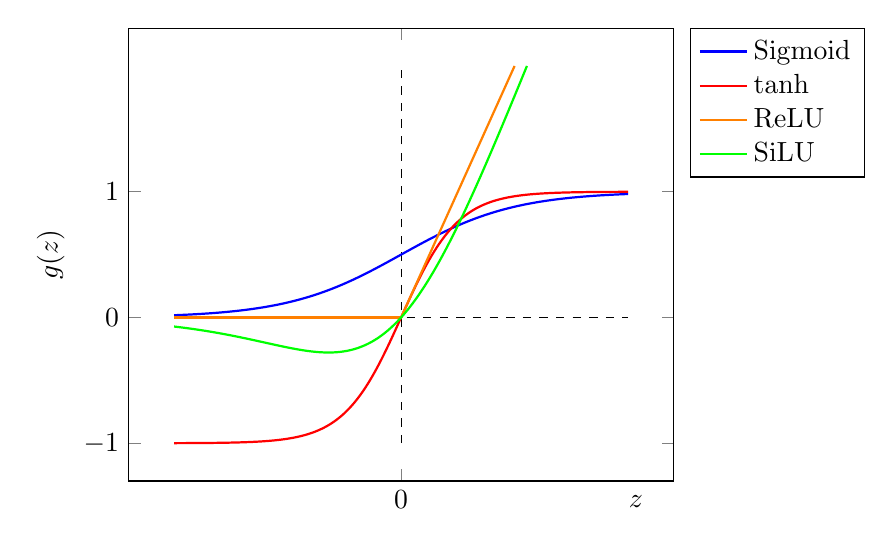
\begin{tikzpicture}
\pgfplotsset{width=8.5cm}
  \begin{axis}[
    domain=-4:4,
    xlabel=$z$,
    ylabel=$g(z)$,
    xtick={0},
    ytick={-1,0,1},
    every axis x label/.style={at={(0.9,-0.01)},anchor=north west},
    legend pos=outer north east,
    legend cell align=left
  ]
  % origin lines
  \addplot +[mark=none, black, dashed, forget plot] coordinates {(-4, 0) (4, 0)};
  \addplot +[mark=none, black, dashed, forget plot] coordinates {(0, -1) (0, 2)};

  % sigmoid 
  \addplot[thick, blue, samples=300] {1/(1+e^(-x))};%
  \addlegendentry{$\textnormal{Sigmoid}$}%

  % tanh
  \addplot[thick, red, samples=300] {tanh(x)};%
  \addlegendentry{$\textnormal{tanh}$}%
  
  % ELU
  %\addplot[thick, blue, samples=300, domain=-4:0, forget plot] {e^x - 1};%
  %\addplot[thick, blue, samples=300, domain=0:2] {x};%
  %\addlegendentry{$\textnormal{ELU}$}%

  % ReLU
  \addplot[thick, orange, samples=300, domain=-4:0, forget plot] {0};%
  \addplot[thick, orange, samples=300, domain=0:2] {x};%
  \addlegendentry{$\textnormal{ReLU}$}%

  % swish 
  % 1.278
  % 2.218
  \addplot[thick, green, samples=300, domain=-4:2.218] {x/(1+e^(-x))};%
  \addlegendentry{$\textnormal{SiLU}$}%

  \end{axis}%
\end{tikzpicture}
  \caption{A diagram displaying the logical flow of a single neuron with 3 inputs. Each neuron can be thought of as a logistic regression model.}
  \label{fig:activation_functions}
\end{figure}

The standard logistic function may not be as quick to train as choices that are asymmetrical about the origin, for example the hyperbolic tangent \cite{efficientbackprop}. The gradient of the activation function dictates how quickly the network can learn - the weight will not change much in areas where the gradient is small. The mean output of a layer with an antisymmetric activation function will be closer to $0$ than for a symmetric activation, and this is where sigmoidal functions have largest gradient. As such, the weight update is more likely to be larger for an antisymmetric function. This is also why data is normalised to have mean and standard deviation equal to 1 in the preprocessing stage.

Another activation function shown to have improvements over both the logistic function and $\tanh$ is the rectifier function. The Rectified Linear Unit (ReLU) were considered.



\subsubsection{Networks}

\subsubsection{Optimisation}


%
\begin{equation}\label{eq:bce_loss}
  J(\bm\theta) = -\frac{1}{m} \sum_{i=1}^m  \mathrm{y}_i \ln[h_\theta(\mathbf{x}_i)] + (1 - \mathrm{y}_i) \ln[1 - h_\theta(\mathbf{x}_i)] .
\end{equation}
%


\subsection{Backpropagation and Gradient Descent}\label{sec:backprop_sgd}

Finally a training algorithm must be developed to allow the program to improve its accuracy through exposure to the dataset. The function $h$ can then be used to predict categories for unseen data. Once the form of $h$ is fixed, the algorithm optimises the coefficients $\bm\theta$ to obtain the best results. The effectiveness of the trained classifier depends on the amount and quality of the training data in $S$, and the efficacy of the training algorithm. The training algorithm works by acting to minimise the \textit{cost function} $J(\bm\theta)$, which gives a measurement of the wrongness of $h$.


gradient descent is an example of an \textit{optimisation} algorithm that minimises the cost function $J(\bm\theta)$ (thereby fitting the logistic regression model discussed above to some data) by selecting the optimal values of $\bm\theta$. The algorithm works by computing the partial derivatives of $J(\bm{\theta})$ with respect to the parameters $\bm{\theta}$. The parameters are then altered slightly in the direction of decreasing slope, thereby reducing the cost function.
%
\begin{equation}\label{eq:weight_update}
    \theta_j \coloneqq \theta_j - \alpha \pd{}{\theta_j} J(\bm\theta)
\end{equation}
%
The parameter $\alpha$ is known as the \textit{learning rate} and dictates the size of the step taken in the direction of the slope. The above step must be performed simultaneously for each $\theta_j$ in $\bm{\theta}$, after which a new value of $J(\bm{\theta})$ can be calculated, and the process repeated. We can compute the partial derivatives of $J$ using the derivative of the logistic function from eq. \ref{eq:bce_loss}. The results are substituted into \cref{eq:weight_update} to obtain
%
\begin{equation}\label{cfpd}
    \pd{J(\bm\theta)}{\theta_j} = \frac{1}{m} \sum_{i=1}^m [h(\mathbf{x}_i) - \mathrm{y}_i] \mathrm{x}_j .
\end{equation}
%
There are many extensions and variations of the gradient descent algorithm. Some examples that provided better results in this project are described briefly below.
%
\begin{itemize}
    \item \textbf{Stochastic gradient descent} (SGD) performs a weight update after exposure to a fixed number of training examples, called a ``batch''. As such the cost function used is an approximation to eq. \cref{eq:bce_loss}. Standard gradient descent is unsuited to large datasets, and SGD has the advantage of introducing randomness from the approximation which means it can escape from local minima \cite{stochasticgrad}.
    %\item \textbf{Adaptive gradient descent} (AdaGrad) adds a learning rate for each weight in the network, so that neurons can learn at individual rates. Built into the algorithm is a reduction in step size over time, so learning slows as training progresses. This encourages good convergence \cite{adagrad}.
    \item \textbf{Adaptive Momentum} (Adam) accelerates SGD by dampening oscillations. A fraction of the previous weight update is used in the current update giving the process ``momentum'' \cite{2014arXiv1412.6980K}.
    %\item \textbf{RMSProp} is a variation of AdaGrad that removes the restriction that the learning rate must be reduced over time. Instead the learning rate depends only on a fixed number of the most recent gradients, and hence the value it can take is more flexible.
\end{itemize}





\section{Track Truth Origin Labelling}\label{sec:track_labelling}

Crucial to supervised learning techniques are are the ground truth class labels which the machine learning model is trained to predict.
, which are listed in \cref{tab:truth_origins}.

\begin{table}[!htbp]
    \footnotesize\centering
    \setlength{\tabcolsep}{0.5em} % for the horizontal padding
    \begin{tabular}{lll}
        \toprule 
        \textbf{Truth Origin} & \textbf{Description} \\
        \hline
        Pileup  & From a \pp collision other than the primary interaction \\
        Fake    & Created from the hits of multiple particles \\
        Primary & Does not originate from any secondary decay \\
        fromB   & From the decay of a \bhadron \\
        fromBC  & From a \chadron decay which itself is from the decay of a \bhadron \\
        fromC   & From the decay of a \chadron which is not from teh decay of a \bhadron \\
        %fromTau & From the decay of a $\tau$ \\
        OtherSecondary & From other secondary interactions and decays \\
        \bottomrule
    \end{tabular}
    \caption{
      Truth origins which are used to categorise the physics process that led to the production of a track.
      Tracks are matched to charged particles using the truth-matching probability~\cite{PERF-2015-08}.
      A truth-matching probability of less than $0.5$ indicates that reconstructed track parameters are likely to be mismeasured and may not correspond to the trajectory of a single charged particle.
      The ``OtherSecondary'' origin includes tracks from photon conversions, \Kshort and $\Lambda^0$ decays, and hadronic interactions.
    }
    \label{tab:truth_origins}
\end{table}

For the fake track classifier, the origins in \cref{tab:truth_origins} are used to construct a binary label by labelling all fake tracks which are not also fromB as background, and all other tracks (i.e. good tracks and fake fromB tracks) as signal.
The fake track classifier is then trained to distinguish between these two categories of tracks.
Fake tracks are defined using the \textit{truth-matching probability} (TMP), defined in \cref{eq:tmp_def}.
This is a weighted sum of the number of hits on a track which are from the same truth particle, versus the total number of hits on the track.
The weights are subdetector-dependent are designed to account for the varying number of layers in each of the subdetectors.
%
\begin{equation}\label{eq:tmp_def}
    \textnormal{TMP} = 
    \frac{
        10 N_{\textnormal{Pix}}^{\textnormal{good}} + 
        5  N_{\textnormal{SCT}}^{\textnormal{good}} + 
           N_{\textnormal{TRT}}^{\textnormal{good}}
        }{
        10 N_{\textnormal{Pix}}^{\textnormal{all}} + 
        5  N_{\textnormal{SCT}}^{\textnormal{all}} + 
            N_{\textnormal{TRT}}^{\textnormal{all}}
        }
\end{equation}
%


\section{Fake Track Identification Tool}\label{sec:fake_track_mva}


The rate of fake tracks increases at high transverse momentum as shown in \cref{fig:fakerate_vs_pt} due to the difficulties in track reconstruction outlined in \cref{sec:b_track_reco_challenges}.
Correspondingly, the performance of \btagging algorithms is reduced, as shown for SV1 in \cref{fig:sv1_perf_nofake}.

\begin{figure}[!htbp]
    \centering
    \includegraphics[width=0.5\textwidth]{chapters/track_classifier/figs/fakerate_vs_pt.pdf}
    \caption{
      Rate of fake tracks as a function of jet transverse momentum.
      The rate of fake tracks increases significantly as a function of \pt, and also increases as the distance to the jet axis decreases, and the number of tracks in the jet increases (not shown).
    }
    \label{fig:fakerate_vs_pt}
  \end{figure}
  
\begin{figure}[!htbp]
    \centering
    \includegraphics[width=0.7\textwidth]{chapters/track_classifier/figs/sv1_perf_nofake.pdf}
    \caption{
      The \ljet efficiency of the low level tagger SV1 as a function of \bjet efficiency for the nominal tracking setup (black) and for the case where fake tracks which are not from the decay of a \bhadron are removed.
      The \ljet efficiency is decreased, demonstrating that the presence of fake tracks is detrimental to algorithm performance.
    }
    \label{fig:sv1_perf_nofake}
  \end{figure}


\section{Conclusion}
todo: culmination of this work in the general classifier tool

Applications:
\begin{itemize}
    \item Frack to jet association
    \item Fake track studies (removal and for recommendations)
\end{itemize}

Improved with GNNs
  \chapter{Graph Neural Network Flavour Tagger}\label{chap:gnn_tagger}

\tofill{Import note}

\section{Graph Neural Network Motivation \& Theory}\label{sec:gnn_motivation_theory}
\section{Model Architecture}\label{sec:gnn_arch}
\section{Results}\label{sec:gnn_results}
\subsection{\btagging Performance}\label{sec:gnn_btag_perf}
\subsection{\ctagging Performance}\label{sec:gnn_ctag_perf}
\subsection{Vertexing Performance}\label{sec:gnn_vert_perf}
\subsection{Track Classification Performance}\label{sec:gnn_tc_perf}

  \chapter{VHbb Boosted Analysis}
\label{chap:vhbb_boosted}

\section{Overview}

\section{Modelling Work}

\subsection{Background}
%
%
\begin{table}[ht]
    \footnotesize\centering
    \setlength{\tabcolsep}{0.5em} % for the horizontal padding
    \begin{tabular}{c|c}
        \hline\hline
        \textbf{Source of Uncertainty}      & \textbf{Implementation} 
        \\
        \hline\hline
        Renormalisation scale ($\mu_R$)     & Internal weights 
        \\
        Factorisation scale ($\mu_F$)       & Internal weights 
        \\
        PDF set                             & Internal weights
        \\
        $\alpha_S$ value                    & Internal weights
        \\
        Parton Shower (PS) models           & Alternative samples 
        \\
        Underlying Event (UE) models        & Alternative samples 
        \\
        Resummation scale (QSF)             & Parameterisation
        \\
        CKKW merging scale                  & Parameterisation
        \\
        \hline
    \end{tabular}
    \caption{Different sources of uncertainty (i.e. variations in the model) considered for V+jets background, and the corresponding implementation. For each uncertainty, acceptance and shape uncertainties are derived.}
    \label{tab:sources of uncertainty}
\end{table}
%
%
\subsubsection{Alternative Samples}
As mentioned, alternative samples of V+jets events was generated using \textsc{MadGraph5\_aMC@NLO+Pythia8}, and the results are compared with the nominal \textsc{Sherpa 2.2.1} samples. This allows for a comparison of different parton showering and underlying event models, and derivation of the systematic uncertainties on the nominal choice of models.

\subsubsection{Internal Weight Variations}
Nominal signal samples generated with \textsc{Sherpa 2.2.1} include systematic variations of certain modelling parameters which are stored as alternative event weights. The samples contain event weight variations which correspond to variations of renormalisation scale $\mu_R$, and factorisation scale $\mu_F$, of $0.5$ and $2$ times the nominal value. Additionally stored is event weight variations corresponding to $30$ different variations on the PDF and two variations of the strong coupling constant $\alpha_S$. Variations of $\alpha_S$ were found to have negligible impact on the results of the analysis, and are not discussed further. 

\subsubsection{Parameterisation Methods}
While the inclusion of internal weight variation in MC event generators has decreased simulation times and increased available statistics, there are in \textsc{Sherpa 2.2.1} currently some sources of systematic uncertainty that are unable to be stored as internal weight variations due to technical limitations. Two such systematics relate to the choice of CKKW matrix element merging scale, and resummation scale (QSF). The generation of high statistics alternative samples is a time consuming process, as is typically not done for all samples for every new generator release. A method to parameterise the systematic variation using one sample, and to then apply this parameterisation to another sample, has been developed by the ATLAS SUSY group \cite{Anders:2125718}. This method was used to derive CKKW and QSF uncertainties for the nominal \textsc{Sherpa 2.2.1} sample, using a previous (lower statistic) \textsc{Sherpa 2.1} alternative sample. The resulting uncertainties were studied and found to be negligible in comparison with systemics from other sources.

\subsubsection{Shape Uncertainties}
In order to derive shape uncertainties (which as the name suggests affect shapes but not overall normalisations of distributions), the following procedure is carried out. Normalised distributions of the reconstructed Higgs candidate mass $m_J$ are compared for the nominal sample and variations. For each variation, the ratio of the variation to nominal is calculated, and an analytic function is fit to those sources of variation which have a ratio deviating from unity. If different analysis regions or channels show the same pattern of variation, a common uncertainty is assigned. An example of a significant source of uncertainty, arising from choice of factorisation scale $\mu_R$ is shown in \cref{fig:vhbb muR shape fitted}. An exponential function has been fitted to the ratio of the normalised distributions. Two different analysis regions (medium and high \pTV bins) are shown. The difference of the shape of the variation means that two separate uncertainties have to be added in the fit, and applied individually in each \pTV region. 
%
\begin{figure}[!htbp]
    \centering
    \begin{subfigure}{.5\textwidth}
      \centering
      \includegraphics[width=\textwidth]{chapters/6.vhbb_boosted/figs/1L_Whf_2tag1pfat0pjet_250_400ptv_SRCR_mJ_SysMUR_T_Norm.pdf}
      \caption{}
      \label{fig:vhbb muR shape fitted sub1}
    \end{subfigure}%
    \begin{subfigure}{.5\textwidth}
      \centering
      \includegraphics[width=\textwidth]{chapters/6.vhbb_boosted/figs/1L_Whf_2tag1pfat0pjet_400ptv_SRCR_mJ_SysMUR_T_Norm.pdf}
      \caption{}
      \label{fig:vhbb muR shape fitted sub2}
    \end{subfigure}
    \vspace{-0.5em}
    \caption{Normalised distributions of leading fat jet mass $m_J$ for medium (\cref{fig:vhbb muR shape fitted sub1}) and high (\cref{fig:vhbb muR shape fitted sub2}) \pTV analysis regions for W+heavy-flavour-jets (merged in heavy flavours, high and low purity signal regions) in the 0 lepton channel. The renormalisation scale $\mu_R$ has been varied by a factor of 2 (``1up'') and 0.5 (``1down''). An exponential function has been fit to the ratio.}
    \label{fig:vhbb muR shape fitted}
\end{figure}

\subsubsection{Acceptance Uncertainties}
Several different types of acceptance uncertainties have been calculated. These are implemented as nuisance parameters in the fit and for the most part account for the migration of events between different analysis regions. The list acceptance uncertainties relevant to the V+jets processes are given summarised below.
%
\begin{itemize}
    \item \textbf{Overall normalisation:} only relevant where normalisation cannot be left floating (i.e. determined in the fit).
    %
    \item \textbf{SR-to-CR relative acceptance:} the uncertainty on the normalisation of the signal region due to events migrating between the signal and control regions.
    %
    \item \textbf{HP-to-LP relative acceptance:} the uncertainty on the normalisation of the high-purity (HP) signal region due to events migrating between the high- and low-purity signal regions.
    %
    \item \textbf{Medium-to-high} \pTV \textbf{relative acceptance:} describes any 'shape' effect in \pTV distribution, given that the analysis only uses two \pTV bins (medium and high).
    %
    \item \textbf{Flavour relative acceptance:} for each flavour V$xx$, where $xx\in$ \{bc,bl,cc\} the ratio of V$xx$/Vbb events is calculated. This corresponds to the uncertainty of Vbb events due to the miss-tagging of other flavours V$xx$. 
\end{itemize}
%
The uncertainties on different systematics are summed in quadrature to give a total uncertainty on each region. A summary of the different acceptance uncertainties that were derived in this way and subsequently applied in the fit are given in \cref{tab:Vjets acceptance uncerts}. An effort has been made, wherever possible, to harmonise similar uncertainties across different analysis regions and channels.


\subsection{Vector Boson + Jets Modelling}
The background processes involving $W$ or $Z$ boson decays into leptons (including those in which the $W$ boson arises from a top-quark decay) are collectively referred to as electroweak (EW), or V+jets, backgrounds. W+jets events are most relevant to the 1-lepton channel via the leptonic decay of W$\rightarrow \ell\nu$. In the event of W$\rightarrow \tau\nu$, and subsequent decay of the $\tau$, or the lack of the successful reconstruction of the $e$ or $\mu$, W+jets can also contribute to the 0-lepton channel. Meanwhile, Z+jets contributes primarily to the 0- and 2-lepton channels via the processes Z$\rightarrow \nu\nu$ and Z$\rightarrow \ell\ell$ respectively.

Modelling is used to predict the outcomes of the analysis and to assess the impact of sources of different systematic uncertainty. Signal and background modelling has has primarily consisted of using Monte Carlo (MC) generators to produce simulated events. The uncertainties on the simulated output must be well understood to perform a successful analysis. To achieve this, a set of ``nominal'' samples are first defined as a reference to which different variations can be compared. The nominal samples are chosen as the best possible representation of the underlying physical process. ``Alternative'' samples are used to understand the systematic uncertainties on the nominal samples. To generate an alternative sample, some aspect of the model is varied, and the simulation is re-run. A comparison back to the nominal sample gives a handle on the systematic uncertainty associated with the model parameter which was changed. Detailed information can be found in \cite{Bell:2316951}. In order to access uncertainties associated with the use of MC generators, variations of the data are produced using alternative generators or variation of nominal generator parameters. The variation of nominal generator parameters can in certain cases be implemented using internal weight variations stored alongside the nominal events, and in other cases a new independent sample must be generated. The nominal generator used for V+jets events is \textsc{Sherpa 2.2.1}, while \textsc{MadGraph5\_aMC@NLO+Pythia8} (which uses different parton showering models) is used as an alternative generator. As production of large MC samples is computationally expensive, a feature of state of the art simulation packages is to store some sources of variation as internal event weights, which can be generated alongside the nominal samples, saving computation time. Several sources of uncertainty, summarised in \cref{tab:sources of uncertainty}, have been assessed.

%
\begin{table}[!htbp] 
  \footnotesize\centering
  \setlength{\tabcolsep}{0.5em} % for the horizontal padding
  %\def\arraystretch{1.4} 
  \begin{tabular}{l|c|c|c|c}
      \toprule\hline
      \multicolumn{5}{c}{V+jets Acceptance Uncertainties}            
      \\ \hline
      \textbf{Boson}      & \multicolumn{2}{c|}{\textbf{W}} & \multicolumn{2}{c}{\textbf{Z}} 
      \\ \hline
      \textbf{Channel}    & 0L          & 1L         & 0L         & 2L          
      \\ \hline
      Vbb Norm.           &   30\%      &     -      &     -      &          -  
      \\ \hline
      SR/CR               &   90\%$^\dagger$         & 40\%$^\dagger$ &      40\%     & -         
      \\ \hline
      HP/LP               & \multicolumn{2}{c|}{18\%}             &   18\%      & -         
      \\ \hline
      High/Medium $p_T^V$ &   30\%      & 10\%$^*$       & \multicolumn{2}{c}{10\%}          
      \\ \hline
      Channel Extrap.             &   20\%      &   -        &    16\%    & -
      \\ \hline
      Vbc/Vbb             & \multicolumn{4}{c}{30\%}                       
      \\ \hline
      Vbl/Vbb             & \multicolumn{4}{c}{30\%}                       
      \\ \hline
      Vcc/Vbb             & \multicolumn{4}{c}{20\%}                       
      \\ \hline
      Vcl Norm.           & \multicolumn{4}{c}{30\%}                       
      \\ \hline
      Vl Norm.            & \multicolumn{4}{c}{30\%}                       
      \\ \hline\bottomrule
  \end{tabular}
  \caption{
    V+jets acceptance uncertainties \cite{Dao:2688371}.
    \Wjets SR and CR uncertainties marked with a superscript $\dagger$ are correlated.
    The 1L \Wjets H/M uncertainty marked by $*$ is applied as independent and uncorrelated NPs in both HP and LP signal regions.
    The 0L \Wjets Wbb Norm uncertainty is only applied when a floating normalisation for Wbb cannot be obtained from the 1L channel.
    A 30\% uncertainty for \Zbb norm is applied in the 1L channel when a floating normalisation for \Zbb cannot be obtained from the 0L or 2L channels.
  }
  \label{tab:Vjets acceptance uncerts}
\end{table}
%

\subsection{Diboson Modelling}



\section{Fit Studies}

\subsection{Fit Model}
A global profile likelihood fit is used to extract the signal strength $\mu$ and its significance from the data. This statistical setup treats each bin as a Poisson counting experiment. The combined likelihood over $N$ bins, without considering sources of systematic uncertainty, is given by
%
\begin{equation}
    \mathcal{L}(\mu) = \prod_{i=1}^N \frac{(\mu s_i + b_i)^{n_i}}{n_i!} \exp \left[ - (\mu s_i + b_i) \right],
\end{equation}
%
where $s_i$ ($b_i$) is the expected number of signal (background) events in bin $i$, and $n_i$ is the number of events observed in data in bin $i$. The presence of systematic uncertainties which can affect the expected numbers of signal and background events necessitates the addition of nuisance parameters (NPs), $\theta$, to the likelihood. Each source of systematic uncertainty for V+jets samples discussed in the previous section was implemented as a NP $\theta_j$ in the fit. The presence of NPs modifies the likelihood as 
%
\begin{equation}
    \mathcal{L}(\mu) \rightarrow \mathcal{L}(\mu, \theta) = \mathcal{L}(\mu) \times \mathcal{L}(\theta) ~,~~~~ s_i \rightarrow s_i(\theta) ~,~~~~ b_i \rightarrow b_i(\theta),
\end{equation}
%
where
%
\begin{equation}
    \mathcal{L}(\theta) = \prod_{\theta_j \in \theta} \frac{\exp\left[{-\theta_j^2/2}\right]}{\sqrt{2\pi}}.
\end{equation}
%
Post-fit $m_J$ distributions in the high-purity medium \pTV regions for the 0- and 2-lepton channels are shown in \cref{fig:vhbb postfit plots}. The plots show large falling backgrounds, predominantly made up of W+jets and Z+jets events, and a signal distribution corresponding to the Standard Model Higgs boson peaking around $m_H = 125$ GeV.
%
\begin{figure}[!htbp]
    \centering
    \begin{subfigure}{.5\textwidth}
      \centering
      \includegraphics[width=\textwidth]{chapters/6.vhbb_boosted/figs/Region_BMax400_BMin250_incFat1_Fat1_Y6051_DSRnoaddbjetsr_T2_L0_distmBB_J0_GlobalFit_conditionnal_mu1.pdf}
      \caption{}
      \label{fig:vhbb postfit plots sub1}
    \end{subfigure}%
    \begin{subfigure}{.5\textwidth}
      \centering
      \includegraphics[width=\textwidth]{chapters/6.vhbb_boosted/figs/Region_distmBB_J0_L2_T2_DSR_Y6051_incJet1_Fat1_incFat1_BMin250_BMax400_GlobalFit_conditionnal_mu1.pdf}
      \caption{}
      \label{fig:vhbb postfit plots sub2}
    \end{subfigure}
    \vspace{-0.5em}
    \caption{Post-fit distributions for the 0-lepton (\cref{fig:vhbb postfit plots sub1}) and 2-lepton (\cref{fig:vhbb postfit plots sub2}) channels in the high purity medium \pTV region, obtained in the combined conditional $\mu=1$ fit to data. The last bin of each plot is an overflow bin.}
    \label{fig:vhbb postfit plots}
\end{figure}
%

\section{Conclusion}

Work has been carried out as part of the boosted VHbb analysis group to understand, and implement in the global profile likelihood fit, systematic uncertainties on V+jets samples. This background modelling work is an essential part of the success of the analysis. So far the fit has proved stable with the inclusion of the V+jets uncertainties, and detailed studies are now underway to determine the causes behind any observed pulls of the added NPs. Additional work is ongoing to help with the derivation of uncertainties on diboson samples, another important background. The analysis is already advanced, and is now progressing into its final stages. Publication is expected in the new year.
  \chapter{Conclusion}
\label{chap:conclusion}

\section{Summary}\label{sec:conc-summary}

The current understanding of particle physics contains many unanswered questions, and improving our understanding of the Standard Model is a promising way to attempt to answer some of them.
Key to this understanding is the Higgs Boson, which was first observed only a decade ago and remains under intense scrutiny at the \LHC.
Given it's propensity to decay to heavy flavour \bquarks, reconstructing and identifying \bjets is of crucial importance to improving our understanding in this area.
As discussed in \cref{chap:tracking}, this task becomes increasingly difficult at high transverse momenta.
The work in this thesis demonstrates that even with suboptimal track reconstruction in this regime, it is possible to make algorithmic advancements to the flavour tagging pipeline to improve the identification of \bjets.
This work has impacts for any analysis which relies on the identification of \bjets, including those which are sensitive to the Higgs Boson.

Analysis of \VHbb events was also carried out with \intlumi of \runtwo \ATLAS at \come{13}.
Various background modelling uncertainties were derived and investigations into the fit model were carried out.
The analysis observed a signal strength of 
$\muVH = 0.72 ^{+0.39}_{-0.36} = 0.72 ^{+0.29}_{-0.28} \mathrm{(stat.)} ^{+0.26}_{-0.22} \mathrm{(syst.)}$
corresponding to an observed (expected) significance of $2.1\sigma$ ($2.7\sigma$).
The result was validated using a simultaneous fit to the \VZbb process.



\section{Future Work}\label{sec:conc-future}

Further algorithmic improvements are likely to yield further improved flavour tagging performance.
Aside from these, large improvements to the flavour tagging performance will likely be possible if improvements are made to the \bhadron decay track reconstruction efficiency and accuracy.

At the moment only the tracks from the Inner Detector and kinematic information about the jet are provided as inputs to the tagging algorithms.
In \cref{chap:gnn_tagger} it was shown that the addition of a simple track-level variable corresponding to the ID of the reconstruction lepton to the model improved the performance.
However there is still untapped potential in the form of additional information from the full parameters of the reconstructed leptons (making full use of the Calorimeters and Muon Spectrometer), the calorimeter clusters, and even the low level hits.
Providing such additional inputs to the model is likely to complement the information provided by the tracks and further aid in the improvement of performane.

On the output side, additional auxiliary training objectives may yield improved performance and also help to add to the explainability of the model.
Regression of jet-level quantities such as the transverse momentum and mass, in addition to the truth \bhadron decay length are promising regression targets.

The \GNN architecture can also be readily optimised for new use cases and topologies, as demonstreated by the studies described in \cref{sec:gnn_trig_upgrade}.
For example, a model with only hit-level information provided as inputs could be used for a fast trigger preselection on jets without the need to run the computationally expensive tracking algorithms.
The model could also be repurposed for primary vertexing, or a pile-up jet tagger.
Finally, the tagging of \largeR jets would benefit those analysis that rely on it.

Ultimately analysis which rely on the identification of heavy flavour jets will likely benefit immensely from the improved performance of the flavour tagging algorithms.
For example, the $HH \rightarrow bbbb$ ... 
\todo{make some claim about improved selection effifiency?}
\end{mainmatter}

%% Produce the appendices if there are any
\begin{appendices}
  %% The "\appendix" call has already been made in the declaration
%% of the "appendices" environment (see thesis.tex).
%\chapter{Combining Multiple Triggers}
%\label{chap:appendix:trigger_efficiencies}


\end{appendices}

%% Produce the un-numbered back matter (e.g. colophon,
%% bibliography, tables of figures etc., index...)
\begin{backmatter}
  \begin{colophon}
This thesis was made in \LaTeXe{} using the ``hepthesis'' class~\cite{Buckley:2010:hepthesis}.
\end{colophon}

%% This is the ATLAS note bibliography style - it
%% may be appropriate to use a different one
\bibliographystyle{bibliography/bibstyles/h-physrev} %atlasnote} %
\bibliography{bibliography/thesis}

%% It's nicer to have these lists here rather than at the front - which would
%% make the front matter last far too long. This disobeys the UCL guidelines.
%\listoffigures
%\listoftables

%% If you have time and interest to generate a (decent) index,
%% then you've spent more time on the write-up than the
%% research ;-)
%\printindex

\end{backmatter}

%% Close
\end{document}
